%%%%%%%%%%%%%%%%%%%%%%%%%%%%%%%%%%%%%%%%%%%%%%%%%%%%%%%%%%%%%%%%%%%%%%%%%%%%%%%%%
%																				%
%			Elen4016-Final-Report.tex			%
%																				%
%                       Ntsako Manyike (28 April 2011)							%
%																				%
%           				%
%														%
%                                                                               %
% Note: Minor modifications were made to the original paper                     %
%       by KJ Nixon 2005/10/12 (with permission from the original author        %
%																				%
%%%%%%%%%%%%%%%%%%%%%%%%%%%%%%%%%%%%%%%%%%%%%%%%%%%%%%%%%%%%%%%%%%%%%%%%%%%%%%%%%

\documentclass[10pt,twocolumn]{witseiepaper}

%
% All KJN's macros and goodies (some shameless borrowing from SPL)
\usepackage{KJN}
\usepackage{rotating}
\usepackage{amsmath}

%
% PDF Info
%
\ifpdf
\pdfinfo{
/Title (Active suspension modelling and control)
/Author (Ntsako Kennedy Manyike)
/CreationDate (D:2011041700)
/ModDate (D:200410220900)
/Subject (Final Report)
/Keywords (ABS,)
}
\fi

%%%%%%%%%%%%%%%%%%%%%%%%%%%%%%%%%%%%%%%%%%%%%%%%%%%%%%%%%%%%%%%%%%%%%%%%%%%%%%%
\begin{document}


\title{MODELING AND CONTROL OF AN ANTI-LOCK BRAKING SYSTEM}

\author{Ntsako K. Manyike}

\thanks{School of Electrical \& Information Engineering, University of the
Witwatersrand, Private Bag 3, 2050, Johannesburg, South Africa}



%%%%%%%%%%%%%%%%%%%%%%%%%%%%%%%%%%%%%%%%%%%%%%%%%%%%%%%%%%%%%%%%%%%%%%%%%%%%%%%
%
\abstract{An anti-lock braking system is the most important safety system in the modern car. It allows the driver to bring the car to a halt in the shortest possible time whilst still maintaining control of the car. A IOFBL controller for a quarter car system is developed using state-space methods. A active suspension model is used to provide a reference input to the controller. The system is simulated and results presented.}

\keywords{State-space, ABS, IOFBL, Active suspension, }


\maketitle
\thispagestyle{empty}\pagestyle{empty}


%%%%%%%%%%%%%%%%%%%%%%%%%%%%%%%%%%%%%%%%%%%%%%%%%%%%%%%%%%%%%%%%%%%%%%%%%%%%%%%
%
\section{INTRODUCTION}

The technology of vehicles, especially cars all over the world is continuously evolving. Along with the many advances in the car manufacturing industry, the safety requirement for cars is of paramount importance. The techniques applied to various cars have already improved system stability and passenger safety with the use of several significant control systems, such as anti-lock braking systems (ABS), active suspension systems, traction control systems etc. 

ABS is a system on motor vehicles which prevents the wheel from locking while braking. The purpose of this system is to allow the driver to maintain steering control under heavy breaking and in some situations to shorten braking distance and time. When brakes lock up on wet and slippery roads during a panic stop the driver might lose steering control and the vehicle can spin.

There have been some integrated studies that combined the aforementioned subsystems in order to further enhance vehicle dynamic efficiency. For example, the concept of integrating ABS with active suspension has been introduced and investigated in the work of \cite{Alleyne:1997}. Many theories and design methods for ABS and active suspension systems have been proposed individually over the years. 

The purpose of this paper is to compare the performance of an ABS controller using the output of the active suspension as an input. A closed loop feedback controller is synthesized from non-linear ABS equations using the input-output feedback linearization (IOFBL) method. The IOFBL is discussed in more detail in\cite{Nyandoro2:2011, Iraj:2008}.


%%%%%%%%%%%%%%%%%%%%%%%%%%%%%%%%%%%%%%%%%%%%%%%%%%%%%%%%%%%%%%%%%%%%%%%%%%%%%%%%
\section{BACKGROUND}

The technology of vehicles, especially cars all over the world is continuously evolving. Along with the many advances in the car manufacturing industry, the safety requirement for cars is of paramount importance. The techniques applied to various cars have already improved system stability and passenger safety with the use of several significant control systems, such as anti-lock braking systems (ABS), active suspension systems, traction control systems etc.
 
ABS is a system on motor vehicles which prevents the wheel from locking while braking. The purpose of this system is to allow the driver to maintain steering control under heavy breaking and in some situations to shorten braking distance and time. When brakes lock up on wet and slippery roads during a panic stop the driver might lose steering control and the vehicle can spin out of control.

There have been some integrated studies that combined the aforementioned subsystems in order to further enhance vehicle dynamic efficiency. For example, the concept of integrating ABS with active suspension has been introduced and investigated in the work of \cite{Crolla:1988}. Many theories and design methods for ABS and active suspension systems have been proposed individually over the years. 

The purpose of this paper is to take advantage of ABS combined with active suspensions to further reduce vehicle braking time and stopping distance. A closed loop feedback controller is synthesized from non-linear ABS equations using the input-output feedback linearization (IOFBL) method. The IOFBL is discussed in more detail in\cite{Nyandoro2:2011, Iraj:2008}.

%%%%%%%%%%%%%%%%%%%%%%%%%%%%%%%%%%%%%%%%%%%%%%%%%%%%%%%%%%%%%%%%%%%%%%%%%%%%%%%
\section{SYSTEM MODELING}

The primary objective of designing an ABS controller is to improve the braking time of a car. The car has an initial longitudinal velocity, $v(t_0) = 120$ $km/h $. When the brakes of the car are applied the car has to come to a stop at a time $t_{f}$ i.e. $v(t_f) = 0$ $km/h$. The purpose of the ABS and active suspension modelling is to minimise $t_f$ whilst maintaining car steering and improving passenger comfort during breaking.

\subsection{Mathematical model}

The mathematical model of the ABS model along with the suspension system is developed. The active suspension system is not discussed in detail but results from previous studies of the suspension systems are used. 

\begin{figure}[ht!]
	\centering
		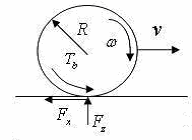
\includegraphics[width=0.50\textwidth]{Quarter_car.png}
	\caption{Quarter car forces and torques \cite{Shaomin:2010}}
	\label{fig:system}
\end{figure}

The model consists of a single wheel of mass $m_u$ and radius $R$ attached to a mass, $m_s$. As the wheel rotates, in the direction of the velocity $v$ driven by the wheels moment of inertia $I$, a tyre reaction force $F_x$ is generated by the friction between the tyre surface $\mu$. The tyre reaction force will generate a torque that initiates a rolling motion of the wheel causing an angular velocity $\omega$. A brake torque $\tau_b$ applied to the wheel will act against the spinning of the wheel causing a negative angular acceleration.

Applying Newton's laws of motion on the quarter car braking model results taking into account that the velocity of the car changes much slower than the other variables involved:

\begin{equation}
	\begin{align}
		m \dot{v} &= -F \mu (\tau)- C_x v^2 \\
		I \dot{\omega} &= -B \omega + F_z \mu (\tau) R - \tau_b \\
		\dot{\tau _b} &= - \frac{1}{\tau}(\tau _b + K_bv_b)
	\end{align}
	\label{eqn:forces}
\end{equation}

where $F_z$ is the total normal force acting on all wheels of the vehicle and $C_x$ is the vehicle aerodynamic friction coefficient. $B$ is the wheel bearing coefficient and $K_b$ is the braking gain. The coefficient of friction $\mu (\tau)$ is a non-linear function of the wheel slip ratio $\tau$. 

During braking, a slippage between the tyre and the contact of the road surface occurs. This slippage can be approximated by: 

\begin{equation}
	\tau = \frac{v - R \omega}{v}
	\label{eqn:slip}
\end{equation}

Equation \ref{eqn:slip} describes the normalised difference between the vehicle speed, $v$ and the wheel perimeter $R\omega$. The coefficient of friction $\mu$ between the tyre and road surface depends on the tyre-road conditions and the value of wheel slip $\lambda$. This value can be worked out experimentally for different road surfaces. The results of which are approximated for dry asphalt, wet asphalt, and icy roads and depicted pictorially in \figref{fig:slip}. From \figref{fig:slip} and Equation \ref{eqn:slip} it is observed that $\lambda = 0$ represents the free rolling wheel condition where no friction force $F_x$ is exerted. While $\lambda = 1$ corresponds to a wheel that is locked ($\omega = 0$). 

\begin{figure}[ht!]
	\centering
		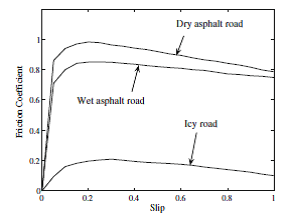
\includegraphics[width=0.50\textwidth]{slip.png}
	\caption{Typical tyre longitudinal friction $\mu$ vs $\lambda$ curves for three types of roads. \cite{Tiem:2008}}
	\label{fig:slip}
\end{figure}

From \figref{fig:slip} it can be seen that the value $\mu (\lambda)$ varies over a wide range of $\lambda$ values. The peak friction coefficient $\mu _0$ occurs at different values of $\lambda$ for the different roads. For higher slip values, the friction coefficient will decrease until the wheel is locked. The function $\mu (\lambda)$  can be approximated by the function:

\begin{equation}
	\mu (\lambda) = 2 \mu _0 \frac{\lambda _0 \lambda}{{\lambda _0} ^2 + \lambda ^ 2}
	\label{eqn:friction}
\end{equation}

where $\mu _0$ is the maximum friction coefficient between the tyre and the road, $\lambda _0$ is the optimal slip ratio which can yield the peak friction value for a specified road. Since $\mu _0 = \mu(\lambda _0)$ then the goal of slip control is to maintain the braking slip value always close or equal to it's optimal value $\lambda _0$ \cite{Pedro:2009}. This reduces the braking distance and ensures the vehicle directional stability during braking.


The normal force $F_z$ on the wheel of the car is the sum of the static and the dynamic weight of the vehicle. The dynamic weight is mainly determined by the longitudinal acceleration of $m_s$. The goal of incorporating the effects of an active suspension system with the ABS modelling and design is so that $F_z$ change in phase with the brake torque $\tau _b$ \cite{Alleyne:1997}. This relationship will ensure that $\mu (\lambda _0)$ occurs at when the brake torque is at it's peak thus resulting in the optimum road brake force. From the complete model, see \cite{Nyandoro1:2011}:

\begin{equation}
	\begin{align}
		m  &= m_s + m_u \\
		F_z &= mg - k_w x_s \\
		F_z &= F_z \mu (\lambda)
	\end{align}
	\label{eqn:suspension}
\end{equation}

Where $k_w$ is the spring constant of the linearized tyre model. Equation \ref{eqn:suspension} shows that the tyre forces $F_z$ and $F_x$ are non-linear functions of the slip ratio $\mu (\lambda)$. This makes the the speed $v$ of the car to be different from the angular wheel speed $\omega$ as will be seen during simulations. Equation \ref{eqn:suspension} shows that the tyre forces are influenced by the static and dynamic force of the car and thus shows that the suspension system does influence the braking performance of the car \cite{Pable:2007}.


%%%%%%%%%%%%%%%%%%%%%%%%%%%%%%%%%%%%%%%%%%%%%%%%%%%%%%%%%%%%%%%%%%%%%%%%%%%%%%%
\section{STATE-SPACE ANALYSIS}

If a linear system can be represented by a set of linear differential equations, then state-space analysis can be used to aid the design of a controller to control the linear system. Since this system is non-linear, IOFBL is to be used for the representation of the system with the aim of synthesising a feedback controller for the system.

%%%%%%%%%%%%%%%%%%%%%%%%%%%%%%%%%%%%%%%%%%%%%%%%%%%%%%%%%%%%%%%%%%%%%%%%%%%%%%%
\subsection{State-space representation}

The goal is to derive a linear multi-input multi-output (MIMO) state-space model for the quarter car set-up. Equations \ref{eqn:forces} - \ref{eqn:suspension}  are non-linear equations. They can be represented in a state-space model as a MIMO system \cite{Nyandoro2:2011}. The states are chosen as \textbf{x} = $[x_1$ $x_2$ $x_3$ $x_4$ $x_5$ $x_6]^T$,  $x_1 = v$, $x_2 = \omega$, $x_3 = x_s$, $x_4 = x_u$, $x_5 = \dot{x_s}$ and $x_6 = \dot{x_u}$.

\begin{equation}
	\begin{align}
		\dot{x} &= f(x)+gu(t) \\
		y &= h(x)=[\lambda \gamma]^T
 	\end{align}
	\label{eqn:iofbl}
\end{equation}

where $\lambda$ is as in Equation \ref{eqn:slip} and $\gamma = x_4 - x_3$, i.e. the suspension travel from the model developed in the laboratory exercise.

%%%%%%%%%%%%%%%%%%%%%%%%%%%%%%%%%%%%%%%%%%%%%%%%%%%%%%%%%%%%%%%%%%%%%%%%%%%%%
\subsection{Input-Output feedback linearisation}

In a non-linear system such as the one presented by Equations \ref{eqn:iofbl}, it is difficult for the output $y(t)$ to track a predetermined  trajectory, $y_d(t)$ while keeping all the $n$ states bounded. This is due to the indirect relationship of the output, $v$, to the input force $\tau _b$ that forces it to $0$. Input-output feedback linearization aims to relate the output with the input via a state \cite{Nyandoro2:2011, Iraj:2008} thus allowing for use of pole placement to design a state variable feedback design. 

This is achieved by differentiating the output equation until $y$ is directly related to the input u. This gives a new linear state equation:

\begin{equation}
  y^r = u_{new}
  \label{eqn:unew}
\end{equation}

With $r$ being the relative degree i.e. the number of differentiations required to relate the input to the output. Equation \ref{unew} represents the stable linearised system. This relationship makes it easy to apply control-law to synthesise a tracking controller. Usually $r < n$ ($n$ = number of states) meaning that some state dynamics are hidden by the linearization process.


%%%%%%%%%%%%%%%%%%%%%%%%%%%%%%%%%%%%%%%%%%%%%%%%%%%%%%%%%%%%%%%%%%%%%%%%%%%%%
\subsection{Feedback controller design}

Feedback control is an error based strategy which regulates the difference between the desired and the achieved output to zero \cite{Sims:1999}. A feedback controller is to be designed using the state-space model. The advantage for the model based model controllers is that they are easy to migrate to different vehicles. 

\begin{figure}[ht!]
	\centering
		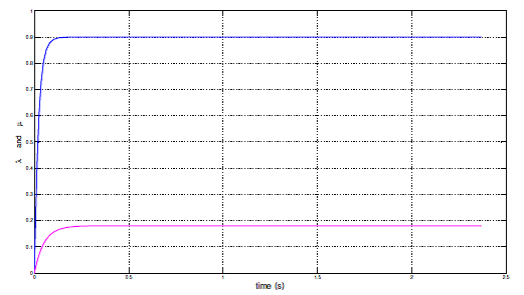
\includegraphics[width=0.50\textwidth]{sliptrack.png}
	\caption{Sample $\lambda$ and $mu$ for ABS with suspension tracking as the input \cite{Nyandoro2:2011}}
	\label{fig:slipTrack}
\end{figure}

During normal driving, the slip ratio $\lambda = 0$. The primary qualitative objective of the slip controller is to bring a car travelling with an initial speed $v(t_0)$ to a halt \cite{Pedro:2009} in the shortest time and distance with the aid of the active suspension system. During braking, the active suspension ABS controller have to improve the ride comfort and keep the slip ratio around the optimal slip ratio $\lambda _0$. \figref{fig:slipTrack} shows a sample $\lambda$ and $\mu$ tracker which is the main goal of the IOFL regulator design. The input to this controller is the dynamic suspension force, $\rho = k_wx_1$ and the suspension travel $\gamma = x_3-x_1$, using the state-space representation.

%%%%%%%%%%%%%%%%%%%%%%%%%%%%%%%%%%%%%%%%%%%%%%%%%%%%%%%%%%%%%%%%%%%%%%%%%%%%%
\subsubsection*{Pole placement for stable linearised system: }

At this point the desired stable closed loop poles can be used to synthesise a state feedback gain matrix \textbf{K}. The poles of the closed loop linearised system are then chosen so that they are asymptotically stable \cite{Nyandoro2:2011}. Simulink is used to determine the poles of \\ \textbf{K} $= [k_{r-1}$ $k_{r-2}$ $...$ $k_0]$ that are stable. This also yields $u$ from Equation \ref{eqn:iofbl}. 

The state feedback matrix is synthesised for a dynamic suspension force $\rho$ acting as the reference input and another one for the suspension travel $\gamma$ as the reference inputs. From this a tracking system for the states can be designed.

%%%%%%%%%%%%%%%%%%%%%%%%%%%%%%%%%%%%%%%%%%%%%%%%%%%%%%%%%%%%%%%%%%%%%%%%%%%%%%%
\subsubsection*{Pole placement for stable linearised tracking system: }

The linearization process has an ultimate goal to allow for the tracking of the desired state. For this particular system the states that are to be tracked are the slip, velocity and linearised angular velocity from the quarter car model shown in \figref{fig:system}. These states are to be tracked for reference input as the suspension force, $\rho$, and the suspension travel, $\gamma$, using the state feedback matrices designed. 

Synthesis of the tracking system is similar to the method used to attain the stabilised pole placement with error dynamics incorporated \cite{Nyandoro2:2011}. Comparing the characteristic equation of $u_{new}$ with the desired closed-loop pole locations the poles of the regulator can be calculated using MATLAB using the command \verb|place| ensuring that the error dynamics go to zero. This is achieved by using the Simulink model provided

%%%%%%%%%%%%%%%%%%%%%%%%%%%%%%%%%%%%%%%%%%%%%%%%%%%%%%%%%%%%%%%%%%%%%%%%%%%%%%%
\section{SIMULATIONS}


%Placed Here so as to appear correctly
\begin{table}[ht!]
	\centering
	\caption{Parameters of the quarter car model used for the simulation.}
		\begin{tabular}{lll}
			\hline
          {\msbf Parameter} 	 & {\msbf Parameter} 	& {\msbf Parameter}\\
      \hline
          B = 0.008 $kgm^2/s$		& $m_s$ = 425 kg   				& $B_sym$ = 200\\
          $K_b$ = 0.8 					& $m_u$ = 40 kg						& $B_{snl}$ = 235..\\
          $T_{max}$ = 10 kNm		& $k_s$ = 23500						& $B_{snl}$ = 400\\
          $T_s$ = 0.45				  & $B_s$ = 700			 				& $J \approx 1.6$ $kdm^2$\\
          $\mu_0$ = 0.8					& $\gamma _{max}$ = 5 mm	& $C_x$ = 0.856 kg/m\\
          $K_w$ = 190 $kNm^{-1}$	&r = 0.35 m 						& g = 9.81 $ms_2$ \\
      \hline
		\end{tabular}
	\label{tab:parameters}
\end{table}

%%%%%%%%%%%%%%%%%%%%%%%%%%%%%%%%%%%%%%%%%%%%%%%%%%%%%%%%%%%%%%%%%%%%%%%%%%%%%%%
\section{RESULTS AND DISCUSSIONS}

The combined ABS and active suspension system dynamics are simulated over a road which has an optimal value of $\mu$. The ABS model used fed with the $\rho$ and $\lambda$ as the reference inputs and the results are presented below. The parameters used in the model are tabulated in Table \ref{tab:parameters}. The simulations track the velocity, wheel angular velocity and displacements for less than 4 s. This is due to the fact that for small velocities, i.e $v < 4m/s$ the simulations break down as shown in \cite{Wright:1984}. 

\begin{figure}
	\centering
		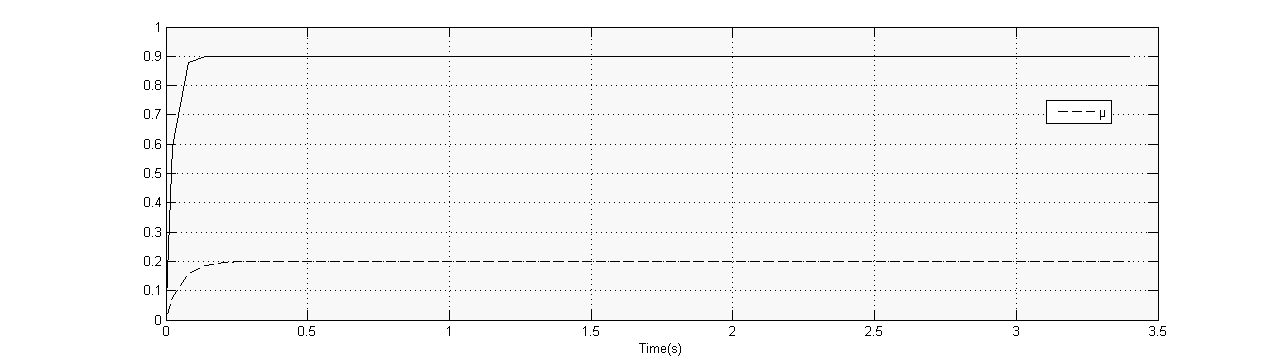
\includegraphics[width=0.50\textwidth]{tracker.png}
	\caption{Slip tracking}
	\label{fig:contrSlip}
\end{figure}

\begin{figure}
	\centering
		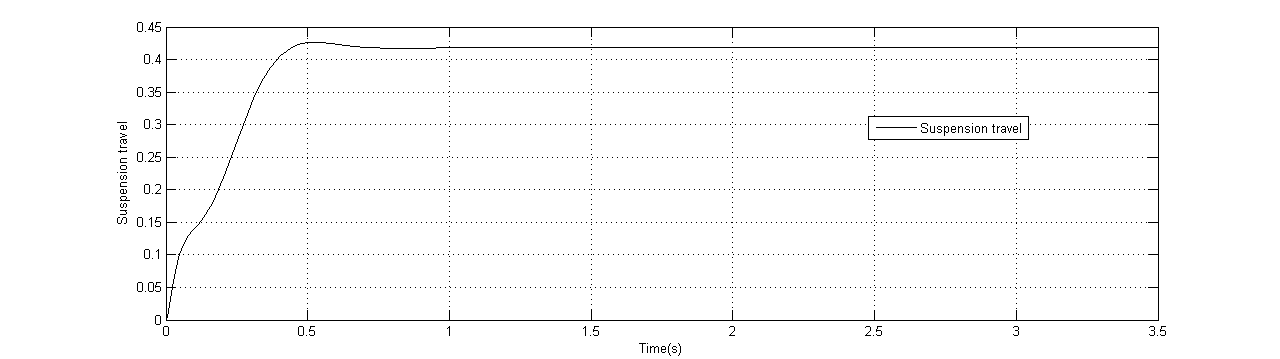
\includegraphics[width=0.50\textwidth]{suspension_travel.png}
	\caption{Suspension travel used as input}
	\label{fig:suspTravel}
\end{figure}

\begin{figure}
	\centering
		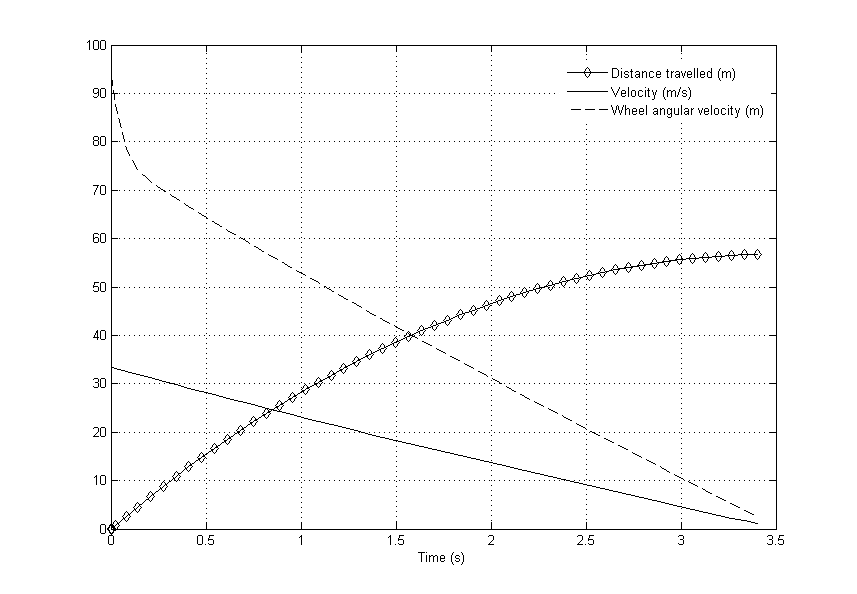
\includegraphics[width=0.50\textwidth]{rho_simulation.png}
	\caption{Time response of breaking speeds and distance.}
	\label{fig:speeds}
\end{figure}

The controllers performance is best tested during braking. A braking torque is applied to the ABS system with the the suspension travel and dynamic suspension forces being the inputs. When the simulations are performed it was found that the suspension dynamic force took less time to arrest the motion of the car than the suspension travel. 

\figref{fig:contrSlip} shows that the controller is is able to track the slip quiete well. The rising time for the slip to reach its optimum point being the only time that the slip is being tracked incorrectly. The travelled distance, car velocity and wheel angular velocity are also plotted in \figref{fig:speeds}. This results show that the car comes to a stop when under the influence of the brake torque and the reference input, $\gamma$.

Looking at the suspension travel, \figref{fig:suspTravel} it is observed that the ride comfort is improved. 

Comparing these controller to the one synthesised in \cite{Shaomin:2010}, it is found that the performances are comparable. In \cite{Shaomin:2010} a sliding mode controller is used on a semi-active suspension with ABS. The comparable results could be also due to the fact that \cite{Shaomin:2010} also considered the road profile and the non-linear tyre in their control. Better performance is achieved by using a fuzzy logic and neural network controller as in \cite{Wang:2009} and \cite{Tiem:2008}. 

Using the MATLAB functions, \verb|ctrb(A,B)| and \verb|obsv(A,C)| on the system model then finding their rank it is found that the system is controllable and observable. Controllability is a vital test on a system to determine if it is worth building a controller for it.

%%%%%%%%%%%%%%%%%%%%%%%%%%%%%%%%%%%%%%%%%%%%%%%%%%%%%%%%%%%%%%%%%%%%%%%%%%%%%%%%%
\section{CONCLUSION}

A IOFBL ABS controller is designed and simulated using state-space techniques. This controller was simulated using Simulink. The simulation includes checking how well the system keeps the value of the slip as close as possible to the optimum slip. It is found that using dynamic actuator forces as a reference input to the ABS system brings the car to a stop quicker.

%\nocite{*}

\bibliographystyle{witseie}
\bibliography{references}

%%%%%%%%%%%%%%%%%%%%%%%%%%%%%%%%%%%%%%%%%%%%%%%%%%%%%%%%%%%%%%%%%%%%%%%%%%%%%%%


%{\tiny \vfill \hfill \today \hspace{5mm} witseie-paper-2003.\TeX}

\end{document}

" vim: ts=4
" vim: tw=78
" vim: autoindent
" vim: shiftwidth=4

